% Gemini theme
% https://github.com/anishathalye/gemini

\documentclass[final]{beamer}

% ====================
% Packages
% ====================

\usepackage[T1]{fontenc}
\usepackage{lmodern}
\usepackage[size=custom,width=120,height=72,scale=1.0]{beamerposter}
\usetheme{gemini}
\usecolortheme{gemini}
\usepackage{graphicx}
\usepackage{booktabs}
\usepackage{tikz}
\usepackage{pgfplots}
\pgfplotsset{compat=1.14}
\usepackage{anyfontsize}
\usepackage{media9}
\usepackage{amsmath}
\usepackage{array}
\usepackage{booktabs}
\usepackage{enumerate}



% ====================
% Lengths
% ====================

% If you have N columns, choose \sepwidth and \colwidth such that
% (N+1)*\sepwidth + N*\colwidth = \paperwidth
\setbeamerfont{itemize item}{size=\fontsize{21pt}{27pt}} % Double itemize items font size
\setbeamerfont{itemize subitem}{size=\fontsize{21pt}{27pt}} % Double subitemize items font size
\setbeamerfont{block title}{size=\fontsize{25pt}{31pt}} % Double block titles font size
\setbeamerfont{block body}{size=\fontsize{21pt}{27pt}} % Double block bodies font size
\setbeamerfont{caption}{size=\fontsize{17pt}{23pt}} % Double figure captions font size

\newlength{\sepwidth}
\newlength{\colwidth}
\setlength{\sepwidth}{0.025\paperwidth}
\setlength{\colwidth}{0.3\paperwidth}

\newcommand{\separatorcolumn}{\begin{column}{\sepwidth}\end{column}}

% ====================
% Title
% ====================

\title{The effects of varying spill hole size on parachute performance}

\author{Carson Thomas}

\institute[shortinst]{Albert Park College}

% ====================
% Footer (optional)
% ====================

\footercontent{
  \href{https://github.com/Technically-Not-The-Worst/Physics-Simulation}{Click for the code of the physics simulations} \hfill
  \href{mailto:carsonthomas@albertpark.vic.edu.au}{carsonthomas@albertparkcollege.vic.adu.au}}
% (can be left out to remove footer)

% ====================
% Logo (optional)
% ====================


% use this to include logos on the left and/or right side of the header:
% \logoright{\includegraphics[height=7cm]{logo1.pdf}}
% \logoleft{\includegraphics[height=7cm]{logo2.pdf}}

% ====================
% Body
% ====================

\begin{document}

\begin{frame}[t]
\begin{columns}[t]
\separatorcolumn

\begin{column}{\colwidth}

  \begin{block}{Introduction}

    Parachutes have been used as a practical means of slowing one's fall for hundreds of years. The optimisation of a parachute comes down to many factors; its size, shape, material and its spill hole. In this investigation aim to standardise all of these variables except for the size of the spill hole, and in doing so I aim to find the relationship between the size of the spill hole and the performance of the parachute. Each of the test will be done with the same base parachute with increasing size spill holes in the centre. I expect the average time of the tests to be inversely proportional to the size of the spill hole. I also expect the consistency of the parachute to roughly proportional to the spill hole size up until a plateau. In essence I hypothesise that due to the larger surface area of the parachutes with smaller spill holes they will fall slower due to the greater induce drag, but the spill holes will introduce a uniform space for air to flow making the parachutes more stable and consistent.

  \end{block}

  \begin{block}{Method}
For this experiment the independant variable will be the radius and hence size of the spill. This means that the parachutes will have to be identical in all other factors. 

    \begin{itemize}
      \item \textbf{Parachute geometry:} all parachutes will be the same shape and size, circles of radius 105mm
      \item \textbf{Parachute material:} each parachute must be made of the some material, A4 printer paper
      \item \textbf{Attached mass:} the mass that is attached to each of the masses must be the same, 50g
       \item \textbf{Drop height:} the height that each parachute must be the same across all drops, 9m 
    \end{itemize}

With those factors being identical across parachutes the one thing changing will be the size of the spill hole. In this experiment there will be 11 parachutes total, 1 control with no spill hole and 10 with increasingly large spill holes. The parachutes will have the spill holes which will be measured by there radius, this radius will increase incrementally by 5mm. Each parachute will use string to attach the 50g mass to 4 points on the parachute equal distances apart on the parachutes. Each parachute shall be dropped from the edge of the balcony at 9 meter and shall be timed from the moment of release to the moment of impact with the ground.

\begin{enumerate}
    \item Ensure that all parachutes are identical in terms of material, shape, and overall size, except for the size of the spill hole.
    
    \item Prepare 11 parachutes in total: 1 control parachute with no spill hole and 10 parachutes with spill holes of varying sizes.


    \item Measure the spill holes by their radius, starting with a radius of 5mm, and increase the radius incrementally by 5mm for each subsequent parachute.

    \item Attach a 50g mass to each parachute using string. The strings should be tied to 4 points on the parachute, evenly spaced and at equal distances apart.

    \item Drop each parachute from a height of 9 meters (e.g., from the edge of a balcony).
    
    \item Time each parachute from the moment it is released to the moment it makes contact with the ground.

    \item Record the time for each parachute to analyze the effect of the spill hole size on the parachute's descent time.
\end{enumerate}


  \end{block}
\begin{alertblock}{The physics at play}
\begin{columns}[t]
\hspace{20pt} % Adjust the value as needed for spacing
\begin{column}{0.5\colwidth}
\begin{itemize}
\setlength{\itemsep}{2mm}
\item
\textbf{Acceleration of gravity: } $F_g = mg$
\item
\textbf{Force of drag: } $ F_{drag} \propto v^2$ 
\item
\textbf{Force of drag: } $ F_{drag} = \frac{1}{2} C \rho Av^2$ 
\item
\textbf{Net acceleration: } $ a = g - \frac{1}{2m} C_d \rho A v^2$ 
\item
\textbf{Terminal velocity: } $ v_{term} = \sqrt{\frac{2mg}{C_d \rho A}}$ 
\item
\textbf{Velocity (with drag): } $ v(t) = v_{\text{term}} \tanh \left( \frac{gt}{v_{\text{term}}} \right)$
\item
\textbf{Height (with drag): } $ h(t) = h_0 - \frac{v_{\text{term}}^2}{g} \ln \left(\cosh \left( \frac{gt}{v_{\text{term}}}\right) \right)$
\end{itemize}
\end{column}
\hspace{10pt} % Adjust the value as needed for spacing
\begin{column}{0.5\colwidth}
\vspace{-13.2pt} % Adjust this value to align the key with the equations
\begin{itemize}
\setlength{\itemsep}{2mm}
\item
\textbf{Key:}
\item $F_g$: Force of gravity
\item $m$: Mass (kg)
\item $C$: Drag coefficient
\item $\rho$: Density of fluid (1.225 kg/m³)
\item $A$: Cross-sectional area (m²)
\item $v$: Velocity (m/s)
\item $g$: Acceleration due to gravity (9.81 m/s²)
\item $C_d$: Coefficient of drag
\item $t$: Time (s)
\item $h_0$: Height offset, beginning height (9m)
\end{itemize}
\end{column}
\end{columns}
\
\end{alertblock}
\end{column}

\separatorcolumn

\begin{column}{\colwidth}

\begin{block}{The Simulations}
Using the equations listed prior and discrete approximations of them (using time steps of 0.001 seconds), I created a simulation to predict the time each drop would take. With these simulations, I created the predicted height and velocity against time graph for each of the parachutes, which you can see below in Figure~\ref{fig:example}. The simulations can be customized by the same variables as the equations, but for this use, only two need to be changed: $A$ (Cross-sectional area) and $C$ (Drag coefficient). The cross-sectional area decreases as the hole in the center increases, and the drag coefficient also changes because the geometry of the parachute changes, affecting how it interacts with the fluid medium. While the area is easily calculated, finding the drag coefficient without CFD software was challenging, so I used educated guesses based on research. If I had access to CFD, the predictions would be more accurate, but this is the best approximation given the resources available.

\begin{columns}

    % First column for the table
    \begin{column}{0.5\textwidth}  % Corrected from \colwidth to \textwidth
        \begin{table}
        \centering
        \begin{tabular}{cccc}
        \toprule
        \textbf{Hole Radius (mm)} & \textbf{Cd} & \textbf{End Time (s)} & \textbf{Max Velocity (m/s)} \\
        \midrule
        0  & 1.50 & 2.5701 & 3.9254 \\
        5  & 1.45 & 2.5341 & 3.9971 \\
        10 & 1.40 & 2.4934 & 4.0817 \\
        15 & 1.35 & 2.4482 & 4.1806 \\
        20 & 1.30 & 2.3989 & 4.2951 \\
        25 & 1.25 & 2.3457 & 4.4272 \\
        30 & 1.20 & 2.2888 & 4.5792 \\
        40 & 1.15 & 2.1987 & 4.8475 \\
        45 & 1.10 & 2.1323 & 5.0708 \\
        50 & 1.05 & 2.0636 & 5.3302 \\
        \bottomrule
        \end{tabular}
        \caption{Maximum velocity and end time for varying hole radii and drag coefficients.}
        \end{table}
    \end{column}

    % Second column for the figure
    \begin{column}{0.5\textwidth}  % Corrected from \colwidth to \textwidth
        \begin{figure}
            \centering
            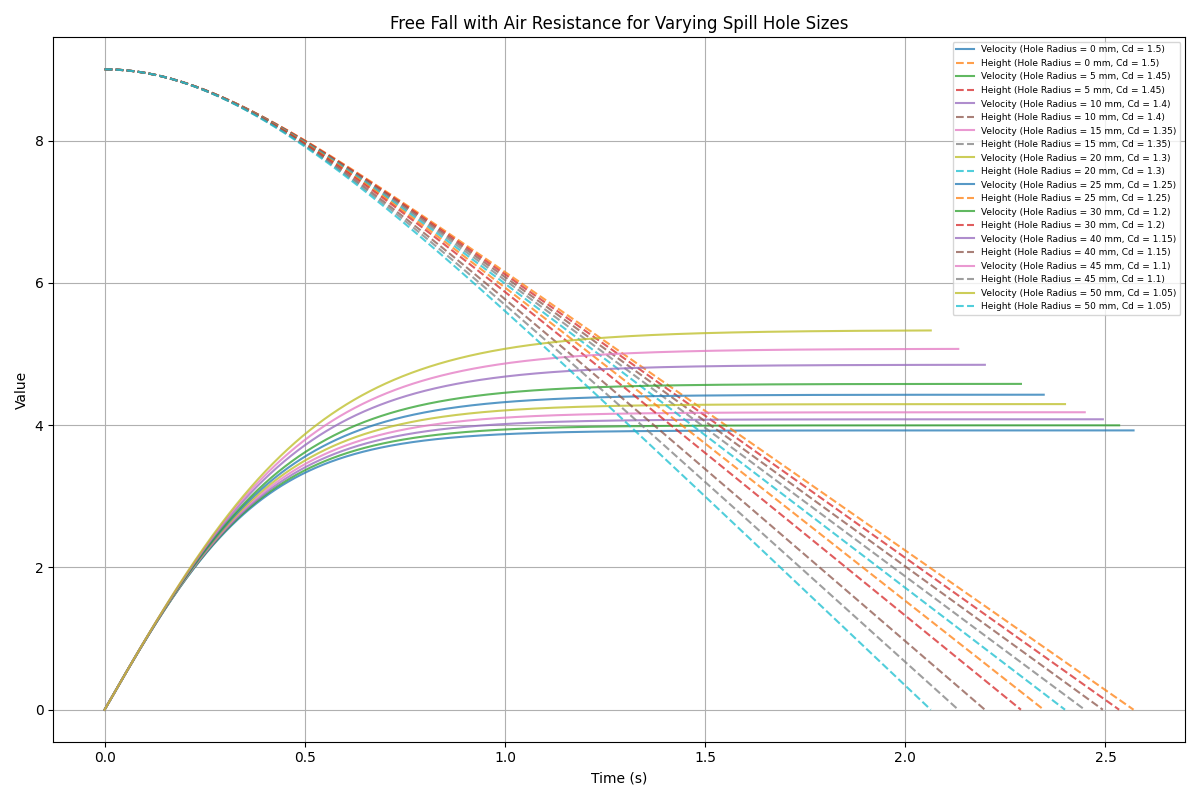
\includegraphics[width=1\linewidth]{/Users/carsonthomas/All_in_one.png} % Ensure image is in the correct directory
            \caption{Height and Velocity against Time.}
            \label{fig:example}
        \end{figure}
    \end{column}

\end{columns}

\end{block}


  \begin{block}{Experimental results}
\begin{columns}[t]
\hspace{20pt} % Adjust the value as needed for spacing
\begin{column}{0.5\colwidth}
\begin{table}[h!]
    \centering
    \begin{tabular}{>{\itshape}c c c c c c}
        \toprule
        Hole Diameter & Run 1 & Run 2 & Run 3 & Avg & Var \\
        \midrule
        0  & 2.68 & 2.30 & 2.48 & 2.49 & 0.03613 \\
        5  & 2.30 & 2.55 & 2.03 & 2.29 & 0.06763 \\
        10 & 2.01 & 2.28 & 2.38 & 2.22 & 0.03663 \\
        15 & 2.05 & 2.38 & 2.20 & 2.21 & 0.02730 \\
        20 & 2.26 & 2.02 & 2.14 & 2.14 & 0.01440 \\
        25 & 2.14 & 2.28 & 2.01 & 2.14 & 0.01823 \\
        30 & 2.21 & 2.18 & 2.29 & 2.19 & 0.00910 \\
        35 & 2.25 & 2.15 & 2.16 & 2.19 & 0.00303 \\
        40 & 2.09 & 2.20 & 2.12 & 2.14 & 0.00330 \\
        45 & 2.25 & 2.23 & 2.2  & 2.22 & 0.00033 \\
        50 & 2.09 & 2.16 & 2.13 & 2.13 & 0.00123 \\
        \bottomrule
    \end{tabular}
    \caption{Test Results for Varying Spill Hole Radii}
    \label{tab:test_results_variance}
\end{table}

\end{column}
\hspace{10pt} % Adjust the value as needed for spacing
\begin{column}{0.5\colwidth}
\vspace{0pt} % Adjust this value to align the key with the equations   
       \begin{figure}
        \centering
        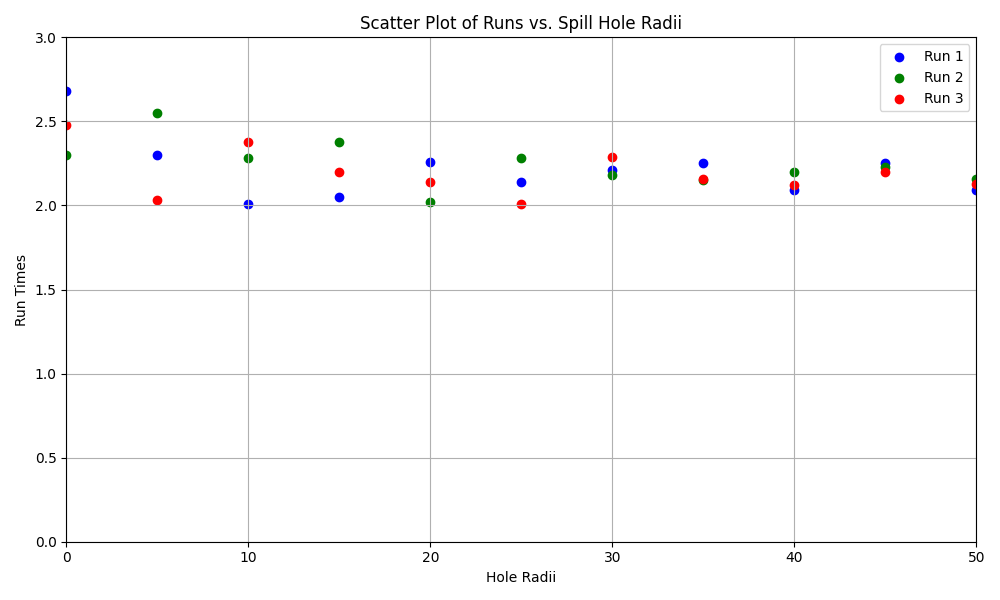
\includegraphics[width=1\linewidth]{/Users/carsonthomas/Desktop/Chart_of_all_runs.png}
        \caption{Height and Velocity Against Time, with moving average.}
        \label{fig:Figure 2}
    \end{figure}
  \end{column}
\end{columns}
\begin{columns}[t]
\hspace{20pt} % Adjust the value as needed for spacing
\begin{column}{0.5\colwidth}
   \begin{figure}
        \centering
        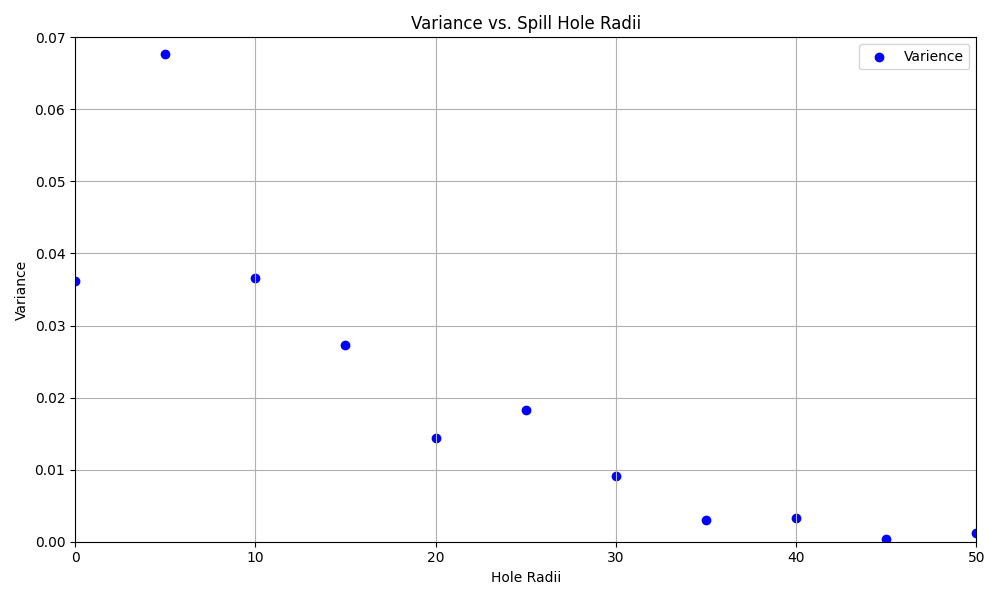
\includegraphics[width=1\linewidth]{/Users/carsonthomas/varience.png}
        \caption{Varience against spill hole radii}
        \label{fig:example}
    \end{figure}
\end{column}
\hspace{10pt} % Adjust the value as needed for spacing
\begin{column}{0.5\colwidth}
\vspace{0pt} % Adjust this value to align the key with the equations   
     \begin{figure}
        \centering
        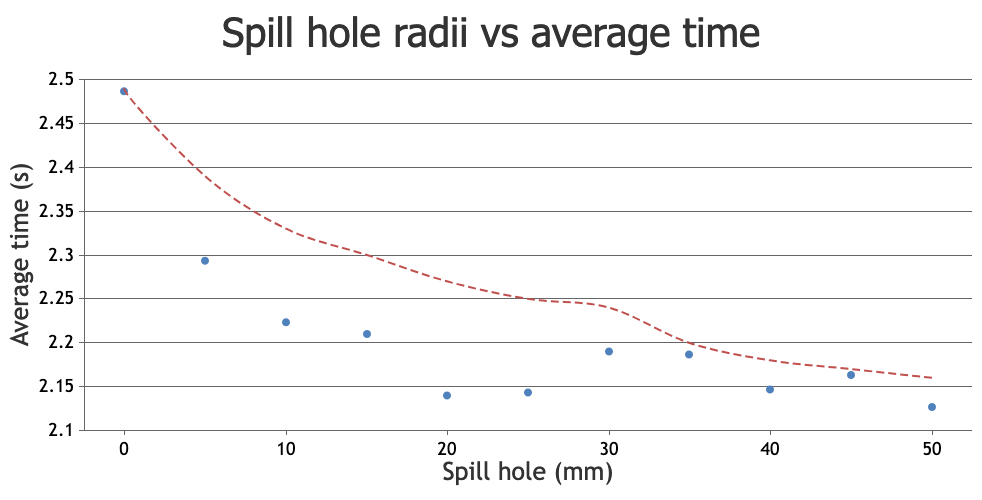
\includegraphics[width=1\linewidth]{/Users/carsonthomas/Downloads/Chart(1).png}
        \caption{Height and Velocity Against Time, with moving average.}
        \label{fig:Figure 3}
    \end{figure}

  \end{column}
\end{columns}
       
  \end{block}



\end{column}

\separatorcolumn

\begin{column}{\colwidth}

  \begin{block}{Discussion}

This study aim to investigate the effects that varying spill hole size has on the efficacy of parachutes. Due to the decrease in cross-sectional area the expected time should decrease as seen in Figure 1 and Table 1, the simulated results show a negative relationship between the spill hole size and the time that the parachute would take to hit the ground. What this demonstrates is that as the cross-sectional area of the parachute decreases and the drag coefficient decreases the time should also decrease. With this in mind as we look to Table 2, Figure 2 and Figure 4 this is what we see, there is a negative trend between the time taken for the parachutes to fall and the size of the spill hole. While the expected results are more linear in nature than the experimental results there is still a negative trend. What the simulations don't speak to is the stability of the parachutes as the  spill hole gets larger. My hypothesis on this relationship would be that as the spill hole gets larger it would create a uniform path for the air to take as the parachute fell creating a more consistent and stable parachute. These increases in consistency and stability should plateau as the spill hole size increases. When looking to Table 2 (Variance) and figure 3 focusing on the variance, a measure of the spread or dispersion within a set of data, one would expect the variance to decrease as the spill hole size increased and this is exactly what we see. In Figure 3 we see a roughly exponential relationship between the spill hole size and the variance, we see a plateau of the decreases in variance with the variance approaching the asymptote of the exponential at zero. The fluid will take the path of least resistance so as a spill hole is introduced it creates a uniform path of least resistance for fluid to take leading to more consistent and stable parachutes. The limitations of this experiment come down to the accuracy of timing, in these runs a stopwatch was used to time from the moment of release to the moment the parachute hit the ground this introduces human error when it comes to the starting and stopping of the timer. Also the simulations used estimated values for the Coefficient of Drag. The accuracy of the timing could be improved by using a camera to record the drop and then count the number of frames the drop took. And the simulation accuracy could be  improved if a CFD was used to find the Coefficient of Drag.
 \end{block}

  \begin{block}{Conclusion}
The aim of this investigation was to find the relationship between the size of a spill hole and the performance of a parachute. This was accomplished by dropping parachutes with increasingly large spill holes and recording the time each took to reach the ground. There was a level of variation in the data from one run to the next and this can be attributed to the human error appearing during the timing of the drops. Due to this human error the validity of the results could be improved, but in spite the human error the results of the experiment were in line with the hypothesis. The study of optimal parachutes is pivotal in creating safe and stable sky diving and supply drops, while on this scale likely having negligible effects on the field. By investigating the optimisation of parachute spill holes more safe and stable parachutes in the future.
  \end{block}

  \begin{block}{References}

\section*{References}

\begin{thebibliography}{9}

\bibitem{Benson2024}
Benson, T. (2024). \emph{The Drag Coefficient}. [online] Available at: \url{https://www.grc.nasa.gov/www/k-12/VirtualAero/BottleRocket/airplane/dragco.html}.

\bibitem{Hoerner1992}
Hoerner, S.F. (1992). \emph{Fluid-dynamic drag: theoretical, experimental and statistical information}. [online] Hoerner Fluid Dynamics. Available at: \url{http://ftp.demec.ufpr.br/disciplinas/TM240/Marchi/Bibliografia/Hoerner.pdf}.

\bibitem{LumenNodate}
Lumen Learning (n.d.). \emph{6.4 Drag Force and Terminal Speed | University Physics Volume 1}. [online] Available at: \url{https://courses.lumenlearning.com/suny-osuniversityphysics/chapter/6-4-drag-force-and-terminal-speed/}.

\bibitem{Lumen2022}
Lumen Learning (2022). \emph{Drag Forces | Physics}. [online] Available at: \url{https://courses.lumenlearning.com/suny-physics/chapter/5-2-drag-forces/}.

\bibitem{PhysicsForums2007}
Physics Forums: Science Discussion, Homework Help, Articles. (2007). \emph{What is the drag coefficient of a square piece of paper in aerodynamics?} [online] Available at: \url{https://www.physicsforums.com/threads/what-is-the-drag-coefficient-of-a-square-piece-of-paper-in-aerodynamics.165775/}.

\bibitem{Tate2010}
Tate, J. (2010). \emph{Gravity Equation}. [online] Universe Today. Available at: \url{https://www.universetoday.com/56157/gravity-equation/}.

\bibitem{Wikipedia2019}
Wikipedia Contributors (2019). \emph{Terminal velocity}. [online] Wikipedia. Available at: \url{https://en.wikipedia.org/wiki/Terminal_velocity}.

\bibitem{Yang2015}
Yang, H., Fan, M., Liu, A. and Dong, L. (2015). General formulas for drag coefficient and settling velocity of sphere based on theoretical law. \emph{International Journal of Mining Science and Technology}, 25(2), pp.219–223. doi:\href{https://doi.org/10.1016/j.ijmst.2015.02.009}{10.1016/j.ijmst.2015.02.009}.
\end{thebibliography}

  \end{block}

\end{column}

\separatorcolumn
\end{columns}
\end{frame}

\end{document}
